\chapter[Implementation]{Implementation}
\label{Chap3}

\section{System Architecture}

The platform developed to visualize atmospheric pollutant forecasts is based on a \textbf{client-only web application running entirely in the browser}. This means that the user does not need to install specialized software or download large datasets to interact with maps and graphs. All interactions occur dynamically and in real time.

The architecture follows a typical pattern for modern web applications. There is a \textbf{presentation layer} responsible for displaying information and enabling user interaction, and a \textbf{data flow} connecting this layer to external services that provide atmospheric data. In this case, the data is offered by CAMS (Copernicus Atmosphere Monitoring Service) through ECMWF’s \emph{ecCharts} platform, which exposes pollutant concentration fields at both global and European scales using the OGC Web Map Service (WMS) standard.

The browser manages interaction and rendering using standard web technologies: HTML for structure, CSS for styling, and JavaScript for interactive logic. Within this layer, \emph{Leaflet} displays interactive maps onto which pollutant layers are overlaid via WMS requests, while \emph{Highcharts} generates on-demand time-series plots of pollutant concentrations at user-selected locations.

For clarity, the architecture can be visualized as illustrated in Figure~\ref{fig:architecture}, the client interacts directly with CAMS servers using WMS requests. The \textbf{web browser} executes the application and issues WMS requests to CAMS servers via the Internet. CAMS servers act as the information provider, rendering pollutant concentration maps (GetMap) and returning pixel values at clicked points (GetFeatureInfo). The data flow is strictly \textit{on demand}: data is only requested when the user selects a pollutant, adjusts the time slider, or clicks on the map.


\begin{figure}[h!btp]
	\centering
	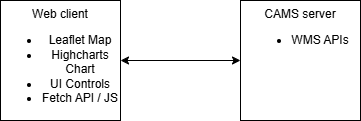
\includegraphics[width=0.6\textwidth]{fig/diagrama1.png}
	\caption{System architecture: interaction between the web client and CAMS servers via WMS APIs.}
	\label{fig:architecture}
\end{figure}

\section{Choice of Mapping Library}

One of the key decisions in the design of the visualization system was the selection of a mapping library capable of rendering geospatial data and providing interactive functionality. This choice is critical because it determines not only the technical possibilities of the system but also its accessibility for future users and developers.  

The first option considered was \textbf{Google Maps API}, a service that is widely recognized and extensively documented. At first sight, it might appear to be the easiest solution, since it provides polished interfaces and reliable infrastructure. However, it is not well suited for the objectives of this project. Being a proprietary tool, it imposes licensing restrictions that limit its free use and redistribution. Furthermore, it offers only limited support for geospatial standards such as WMS (Web Map Service), which are essential when working with scientific or institutional sources of environmental data.  

Another possibility was \textbf{OpenLayers}, an open-source library that is highly regarded in the professional field of web mapping. Its main strength lies in its native compatibility with OGC standards, including WMS, WFS, and WMTS. This makes it an extremely powerful and flexible option for complex applications. Nevertheless, this power comes at the cost of a higher degree of complexity. The learning curve for OpenLayers is steeper, and for a project intended to be both educational and easy to prototype, this could represent an unnecessary barrier for development and future maintenance.  

The final choice was \textbf{Leaflet.js}, a lightweight and widely adopted library for interactive web maps. Although its built-in support for WMS services is more basic than that of OpenLayers, it can be extended with a rich ecosystem of plugins, such as \textit{leaflet.wms} or \textit{leaflet.timeDimension}. These extensions allow seamless integration of external services, including the CAMS datasets used in this project, and make it possible to explore temporal variations in air quality data through interactive layers.  

Leaflet was selected because it offers the best balance between simplicity and functionality. Its design allows developers to build interactive maps with only a few lines of code, accelerating the prototyping process. The library is very lightweight (less than 40~KB), which ensures quick loading times even on devices with limited resources, thereby improving accessibility. Since it is entirely open-source and free to use, it also aligns with the philosophy of this project, which aims to rely on open technologies to guarantee reproducibility and long-term usability. Finally, Leaflet benefits from an active and large community that provides tutorials, documentation, and practical examples, making it easier to learn, troubleshoot, and sustain over time.  

In summary, Leaflet represents an optimal solution for this project. It is powerful enough to handle CAMS WMS layers and interactive visualizations, while remaining simple and approachable for future users or developers who may wish to extend or adapt the tool without requiring advanced expertise in geospatial technologies.  


\section{Discovering Available Layers}

To determine which pollutants and forecast products are available from CAMS, it is necessary to inspect the WMS service capabilities. ECMWF provides documentation of the CAMS WMS service, but the official page does not contain the complete list of layers. Therefore, the full set of available layers is obtained through a \texttt{GetCapabilities} request, which returns an XML document describing them. Each layer entry includes its internal identifier, descriptive title, units (if defined), and the time dimension specifying the forecast horizon.


The process can be automated using a Python script, shown in Listing~\ref{lst:getcapabilities}. It sends a request to the CAMS server, parses the XML, and prints out the available layers with their metadata:

\lstset{language=Python, 
	basicstyle=\ttfamily\small, 
	keywordstyle=\color{blue}\bfseries, 
	commentstyle=\color{gray}\itshape, 
	stringstyle=\color{red}, 
	breaklines=true,
	frame=single,
	numbers=left,
	numberstyle=\tiny,
	captionpos=b
}
 \begin{lstlisting}[language=Python, caption={Python script to extract CAMS layers from WMS GetCapabilities}, label={lst:getcapabilities}]
		import requests
		import xml.etree.ElementTree as ET
		
		url = "https://eccharts.ecmwf.int/wms/?token=public&request=GetCapabilities&version=1.3.0"
		
		response = requests.get(url)
		xml_content = response.content
		
		root = ET.fromstring(xml_content)
		
		ns = {'wms': 'http://www.opengis.net/wms'}
		
		layers = root.findall('.//wms:Layer/wms:Layer', ns)
		
		print(f"Found {len(layers)} layers:\n")
		
		for layer in layers:
		name = layer.find('wms:Name', ns)
		title = layer.find('wms:Title', ns)
		units = layer.find('wms:Units', ns)
		dimension = layer.find("wms:Dimension[@name='time']", ns)
		
		print("Layer:")
		print(f"  Name:   {name.text if name is not None else 'N/A'}")
		print(f"  Title:  {title.text if title is not None else 'N/A'}")
		print(f"  Units:  {units.text if units is not None else 'N/A'}")
		print(f"  Time:   {dimension.text[:50] + '...'}" if dimension is not None else "  Time:   N/A")
		print("-" * 40)
\end{lstlisting}

When executed, the script returns a list of all the layers exposed by CAMS. Each entry contains the pollutant or variable identifier, its description, the units, and the available time stamps. in Listing~\ref{lst:truncatedoutput}.

\begin{lstlisting}[caption={Truncated output of the GetCapabilities request}, label={lst:truncatedoutput}]

	Found 121 layers:
	...
	
	Layer: 
	Name: composition_o3_surface Title: Ozone at surface [ppbv] (provided by CAMS, the Copernicus Atmosphere Monitoring Service)
	Units: N/A Time: 2025-08-23T03:00:00Z,2025-08-23T06:00:00Z/2025-09-... 
	---------------------------------------- 
	
	Layer: 
	Name: 
	composition_europe_o3_analysis_surface 
	Title: Ozone at surface [ug/m3] (provided by CAMS, the Copernicus Atmosphere Monitoring Service) 
	Units: N/A 
	Time: 2022-11-28T00:00:00Z,2022-11-29T00:00:00Z/2023-01-... 
	---------------------------------------- 
	
	Layer: 
	Name: composition_pm10 
	Title: PM10 - coarse particulate matter [ug / m3] (provided by CAMS) 
	Units: N/A 
	Time: 2025-08-23T03:00:00Z,2025-08-23T06:00:00Z/2025-09-... 
	----------------------------------------
	
	...
\end{lstlisting}

This information is essential for dynamically populating the pollutant menu and enabling correct requests for specific forecast hours.


\section{Hourly Forecast Handling}

The platform provides hourly forecasts of atmospheric pollutants, enabling users to explore both the spatial distribution of pollutants on a map and the temporal evolution at specific locations. Handling these hourly forecasts involves several interconnected components, including the time slider, the WMS requests to CAMS, the rendering of map layers, and the visualization of historical data.

The first key component is the time slider, which allows the user to select the forecast hour they wish to inspect. The application automatically calculates the range of available forecast hours based on the current UTC time and a forecast horizon of four days. For each hour within this range, an ISO-formatted timestamp is generated and associated with a position on the slider. When users select a global forecast, the application rounds the chosen hour to the nearest multiple of three, reflecting the temporal resolution of the global CAMS forecasts. The slider also displays labels that indicate the day of the forecast, providing an intuitive reference so users can easily identify which hours correspond to which day.


\section{Conversion of Pollutant Values}

Some of the data layers were not given in \(\mu g/m^3\) (micrograms per cubic meter), but in ppbv (parts per billion by volume).  
To standardize the units, a pollutant-specific conversion factor was applied.  

These factors are derived from the relationship between volumetric concentration and mass using the ideal gas law:

\[
C_{\mu g/m^3} = C_{ppbv} \times \frac{M \cdot P}{R \cdot T} \cdot 10^3
\]

where:
\begin{itemize}
	\item \(C_{\mu g/m^3}\) = concentration in micrograms per cubic meter (\(\mu g/m^3\))  
	\item \(C_{ppbv}\) = concentration in parts per billion by volume (ppbv)  
	\item \(M\) = molar mass of the pollutant (g/mol)  
	\item \(P\) = pressure (Pa)  
	\item \(R\) = universal gas constant \(8.314\,\mathrm{J/(mol\cdot K)}\)  
	\item \(T\) = absolute temperature (K)  
\end{itemize}

The factors used in the code were calculated assuming standard pressure and temperature conditions (\(P = 101325\,Pa\), \(T = 298\,K\)) and applying the equation above.  

\textbf{Note on temperature:} \(T = 298\,K\) corresponds to approximately \(25\,^\circ C\).


For example, for \(\mathrm{NO_2}\):

\[
\mathrm{NO_2\ Factor} = \frac{46.0055\,[g/mol] \cdot 101325\,[Pa]}{8.314\,[J/(mol\cdot K)] \cdot 298\,[K]} \cdot 10^{-3} \approx 1.9125
\]

This means that each ppbv of NO\(_2\) corresponds approximately to \(1.9125\,\mu g/m^3\).  

The code that performs the conversion is:

\lstdefinelanguage{JavaScript}{
	keywords={break, case, catch, class, const, continue, debugger, default, delete, do, else, export, extends, finally, for, function, if, import, in, instanceof, let, new, return, super, switch, this, throw, try, var, while, with, yield},
	morecomment=[l]{//},
	morecomment=[s]{/*}{*/},
	morestring=[b]",
	morestring=[b]'
}
\begin{lstlisting}[caption={Conversion of pollutant values to \(\mu g/m^3\)}]
	function convertPollutantValue(pollutant, rawValue) {
		let value = parseFloat(rawValue);
		let unit = "ug/m3"; 
		
		switch (pollutant) {
			case "NO2": value = value * 1.9125; break;
			case "SO2": value = value * 2.6609; break;
			case "CO":  value = value * 1.1642; break;
			case "CO2": value = value * 1.829; break;
			case "CH4": value = value * 0.666; break;
			case "O3":  value = value * 1.9957; break;
			default: value = value * 1; break;
		}
		
		return { value: Math.round(value * 100)/100, unit };
	}
\end{lstlisting}

Each factor in the code corresponds to the calculation shown for NO\(_2\), adjusted for the molar mass of each pollutant. This ensures all values are in the same unit (\(\mu g/m^3\)) for consistent analysis and comparison.

\section{Dynamic Layer Updating}

Whenever the user changes the selected region, pollutant, or forecast hour, the function \texttt{actualizarCapa()} is triggered. This function is responsible for updating the map with the correct pollutant layer for the chosen time. It first computes the exact time to request from the CAMS servers, taking into account region-specific rounding rules. Using the service URL provided by CAMS, it then constructs a WMS GetMap request, specifying the layer corresponding to the selected pollutant. If a color gradient style is defined for that pollutant, it is included in the request to ensure a meaningful visual representation. Before adding the new layer to the map, any previous pollutant layer is removed, ensuring that only the selected forecast is visible. The map legend is also updated at this point, reflecting the pollutant’s concentration range and the color mapping used to represent different values.


\begin{lstlisting}[caption={Updating the map layer for the selected pollutant and hour}]
	function actualizarCapa() {
		if (wmsLayer) map.removeLayer(wmsLayer);
		
		const layerName = wmsInfo[region].layers[contaminante];
		const wmsUrl = wmsInfo[region].url;
		
		wmsLayer = L.tileLayer.wms(wmsUrl, {
			layers: layerName,
			format: 'image/png',
			transparent: true,
			opacity: 0.6,
			time: timeISO
		}).addTo(map);
		
		if (styleName) wmsLayer.setParams({ styles: styleName });
		
		leyendaDiv.textContent = `Leyenda: ${leyendas[contaminante]} (Hora UTC: ${fechaReal.getUTCHours()}:00)`;
		renderLegend(contaminante);
	}
\end{lstlisting}

\section{Pollutant Value Extraction on Map Click}
Users can click on any point of the map to obtain the forecasted concentration of the selected pollutant at that location. This is accomplished by an asynchronous function, which sends a WMS GetFeatureInfo request to the CAMS servers using the coordinates of the clicked point and the selected forecast hour. The response is parsed to extract the raw pollutant value, which is then converted to a standardized unit using predefined conversion factors specific to each pollutant. The result, including both the concentration and its unit, is displayed on the interface, allowing users to quickly understand the expected air quality at a given location.


\section{Historical Data Visualization}
In addition to showing the concentration at a single point in time, the platform allows users to explore the temporal profile of pollutant concentrations at a specific location. The function \texttt{getHistoricalDataForPollutant()} retrieves data for all available forecast hours in the slider. Each forecast hour is queried individually through a WMS GetFeatureInfo request, and the values are converted to consistent units. The resulting time series is plotted using Highcharts through the \texttt{plotPollutantHistory()} function, producing an interactive line chart. This feature enables users to visualize how pollutant concentrations evolve over time and identify periods of higher risk.


\begin{lstlisting}[language=JavaScript, caption={Plotting historical pollutant data using Highcharts}]
	function plotPollutantHistory(data) {
		Highcharts.chart('chartContainer', {
			chart: { type: 'line', zoomType: 'x' },
			title: { text: 'Historial de Contaminantes' },
			xAxis: { type: 'datetime', title: { text: 'Fecha/Hora UTC' } },
			yAxis: { title: { text: 'Concentracion (ug/m3)' }, min: 0 },
			series: [{ name: contaminanteSelect.value, data: data, turboThreshold: 0 }],
			credits: { enabled: false },
			exporting: { enabled: true }
		});
	}
\end{lstlisting}

\section{Animation of Forecasts}

To further facilitate understanding of pollutant trends, the platform provides a play/stop button that animates the forecast over all available hours. Activating this feature sequentially advances the slider, updating both the WMS layer on the map and the legend in real time. This animation helps users intuitively grasp the dynamics of pollutant distribution and evolution without manually adjusting the slider.

\section{Color Gradients and Legends}

Finally, each pollutant has a predefined color gradient and threshold levels stored in the application. When a layer is displayed, a floating legend is rendered on the screen. This legend visually represents the range of concentrations using the color gradient and indicates key values such as the minimum, 30\%, 50\%, 70\%, and maximum thresholds. Additionally, the legend includes the name of the pollutant and the measurement unit.

The legend is generated by requesting the corresponding WMS layer, which returns an image containing the color gradient and associated threshold levels. From this image, it is posible to extract both the colors and the numerical values for each threshold. These extracted values are then combined with the pollutant-specific conversion factor, ensuring that the legend displayed in the interface matches the standardized units used in the map and in the time-series charts.

This approach ensures consistency between the visual representation of pollutant concentrations and the numerical data displayed, allowing users to intuitively interpret both current and forecasted air quality levels directly from the map.